\documentclass[10pt]{llncs}
\usepackage[utf8]{inputenc}
\usepackage{graphicx}

\begin{document}
\title{Towards Secure Cross-Organizational Data Transfer: A Blockchain-Enabled Message Broker Approach}
\author{Gleb Slepenkov\inst{1}\orcidID{0009-0001-9978-396X}}
\authorrunning{G. Slepenkov}
\institute{Saint Petersburg State University, 7-9 Universitetskaya Embankment, St Petersburg, Russia, 199034}

\maketitle

\begin{abstract}
    Secure data transmission (SDT) is crucial in modern information societies, particularly for cross-organizational data exchange. 
    This paper investigates the application of blockchain technology to create robust SDT systems, combining the benefits of using blockchain as both a data access interface and a direct data transfer tool. 
    We propose a novel architecture featuring a message broker-like design that overcomes data size limitations present in existing blockchain-based SDT solutions. 
    The architecture incorporates blockchain, internal data storage within organizations, and connectors facilitating interaction between these components. 
    The SDT process relies on smart contracts for managing data access, transfer, and confirmation, while the actual data is stored off-chain. 
    We advocate for a private, two-layered blockchain implementation, employing PBFT consensus within smaller clusters for efficient message transfer and RAFT consensus for system management and data replication. This layered approach enhances both fault tolerance and scalability, paving the way for a practical and secure cross-organizational SDT system.
    
    \keywords{Blockchain \and Secure Data Transfer (SDT) \and Data Security \and Distributed Ledger Technology (DLT) \and Message Broker \and Data Access Control \and Cross-Organizational Data Sharing \and Scalability \and Fault Tolerance}
\end{abstract}

\section{Introduction}

In contemporary information societies, secure data transmission (SDT) is paramount for maintaining data confidentiality and integrity.
SDT systems are critical infrastructure components across diverse sectors, including financial institutions, governmental agencies, and enterprises.

Implementing robust SDT mechanisms becomes particularly challenging when facilitating cross-organizational data exchange or connecting geographically dispersed departments within a single organization.
Such scenarios necessitate data transfer across external, public networks, thereby significantly elevating the risk of unauthorized data disclosure or modification during transit.
Consequently, rigorous data integrity verification and sender authentication protocols are indispensable.
Furthermore, confirmation of data reception is often a critical requirement.
The heterogeneity of data exchange technologies employed by different entities can further complicate the SDT process.

Blockchain represents an emerging technology for SDT solutions.
This technology by design provides core features essential for SDT, such as fault tolerance, ledger data immutability and zero trust between blockchain nodes.
Moreover, many blockchains are designed to operate in unreliable public networks with nodes running in different heterogeneous clusters owned by separate stakeholders.
For this reason, blockchains are especially suitable for cross-organizational data transfer.
Furthermore, blockchain platforms often provide smart contracts, which allow implementing custom data transfer logic directly on the blockchain.

This suitability has spurred significant research interest, as evidenced by comprehensive surveys exploring blockchain applications for data sharing and exchange \cite{Song2023} and for specific domains like smart transport \cite{Bagga2022}.
These surveys highlight the potential of blockchain to address the challenges of SDT in diverse and demanding environments.

This study investigates existing paradigms of blockchain applications to the SDT process and proposes a new approach, which allows to combine the advantages of existing paradigms and create 
a SDT blockchain-based system that preserves key features of existing approaches but has a message broker-like architecture and relaxed data size limitations.
The study is organized in the following way.
Section \ref{related_work} describes existing data transfer paradigms in detail.
Section \ref{architecture} represents the proposed system architecture.
Section \ref{implementation_details} describes implementation details of the proposed system.
Finally, Section \ref{summary} concludes this article and denotes further research directions.

\section{Related Work} \label{related_work}

The integration of blockchain technology into data transfer systems presents two primary paradigms: blockchain as a data access interface and blockchain as a direct data transfer tool.
This section examines the existing literature, classifying studies according to these two distinct roles of blockchain in facilitating data exchange.

\subsection{Blockchain as a Data Access Interface}

This approach leverages blockchain as a secure and transparent mechanism for managing and controlling access to data that is typically stored off-chain.
The blockchain records metadata about the data, access permissions, and transaction histories, thereby ensuring data integrity, auditability, and secure access control.
The data itself is transferred using conventional methods.

Wang et al. introduced BBS, a big data sharing system utilizing blockchain for access control and data integrity management \cite{Wang2024}.
Similarly, Wang et al. proposed a blockchain-based model for sharing big data in the oil and gas sector, employing blockchain to enable secure data access and provenance tracking \cite{WangYY2021}.
Yang et al. developed a sharing platform for wild bird data based on blockchain and IPFS, where blockchain governs access rights to data residing in IPFS \cite{Yang2022}.
A cross-organizational data sharing framework that uses blockchain probes to orchestrate and audit data access across various entities was presented by Jia et al. \cite{Jia2023}.
Gupta et al. explored the application of blockchain for securing data access within e-healthcare applications \cite{Gupta2022}.
\subsection{Blockchain as a Data Transfer Tool}

This approach employs the blockchain directly to transfer data between participants.
While data may occasionally be stored on-chain, it is more common for the blockchain to facilitate the transfer of data stored off-chain,
 often in conjunction with technologies such as peer-to-peer networks or distributed file systems.

Lin et al. proposed a multi-level blockchain architecture for secure data transfer in the Internet of Vehicles (IoV), 
directly leveraging blockchain for data exchange \cite{Lin2023}. 
Peng et al. demonstrated the feasibility of building a peer-to-peer file storage and sharing system on a consortium blockchain, 
where the blockchain assists in discovering and securely transferring file chunks \cite{Peng2023}. 
Priyadarshini et al. introduced a system for secured data transfer between fog nodes utilizing blockchain to enhance the security of 
the data transfer process itself \cite{Priyadarshini2021}.

\subsection{Enabling Technologies and Security Considerations}

Regardless of the chosen paradigm, several enabling technologies and security considerations are universally relevant. 
Kim et al. presented a hybrid decentralized PBFT blockchain framework for OpenStack message queues, aimed at improving fault tolerance and scalability, 
crucial aspects for reliable data transfer systems \cite{kim2020hybrid}. 
A publish-subscribe architecture to foster interoperability among different blockchain networks, thus facilitating data exchange across heterogeneous systems, was introduced by Ghaemi et al. \cite{Ghaemi2021}. 
Bagga et al. and Xu et al. explored blockchain-based authentication and key agreement protocols for IoV, enhancing the security of data transfer in vehicular contexts \cite{Bagga2021,Xu2021}. 
Bogdanov et al. focused on the consensus mechanism, exploring a combination of PBFT and Raft \cite{Bogdanov2024}, while Ai et al. proposed a Proof-of-Transactions consensus protocol \cite{Ai2022}, 
both striving for efficient and scalable agreement in distributed ledgers. 

\subsection{Comparison of Approaches}

The two approaches, blockchain as a data access interface and blockchain as a data transfer tool, offer distinct advantages and disadvantages depending on the specific use case and requirements.

\begin{table}[h!]
\caption{Comparison of Blockchain Approaches for Data Transfer}
\label{tab:comparison}
\begin{tabular}{|p{2.0cm}|p{5.0cm}|p{5.0cm}|}
\hline
Feature & Blockchain as Data Access Interface & Blockchain as Data Transfer Tool \\ \hline
Data Storage & Primarily Off-Chain & Often Off-Chain, but metadata on-chain \\ \hline
Data Transfer & Traditional methods & Blockchain or Blockchain-assisted \\ \hline
Scalability & Higher, as data transfer is off-chain & Potentially Lower, dependent on blockchain throughput \\ \hline
Complexity & Lower & Higher \\ \hline
On-Chain Footprint & Smaller (Metadata only) & Larger (Metadata and potentially data chunks) \\ \hline
Suitability & Large datasets, access control focus & Smaller datasets, secure and direct transfer focus \\ \hline
\end{tabular}

\end{table}

As illustrated in Table \ref{tab:comparison}, the choice between these two approaches hinges on factors such as data size, scalability requirements, security priorities, 
and the level of on-chain transparency desired. 
The data access interface approach is generally more suitable for scenarios involving large datasets and a primary focus on secure access control, while the data transfer tool 
approach is better suited for scenarios demanding secure and direct data transfer, even if it potentially introduces limitations in terms of scalability.

\section{Proposed system architecture} \label{architecture}

\subsection{Overview}

This section describes the architecture of the proposed system.
The main goal of such an architecture is to create a combination of the two main blockchain integration paradigms into data transfer systems described in Section \ref{related_work}
in order to create a system with a message broker-like architecture, convenient for data transfer, and relaxed data size limitations compared to existing solutions.
Essentially, the architecture follows the trends described in related articles:

\begin{enumerate}
    \item Blockchain usage as a message broker: \cite{Ghaemi2021}, \cite{kim2020hybrid}. 
    The key drawback of these solutions lies in the usage of the ledger for message transfer.
    It greatly limits the system scalability and transferred data size. 
    \item Blockchain as an interface to off-chain data (e.g., \cite{Jia2023}, \cite{Wang2024}).
    Such solutions usually do not have any notification mechanisms.
    Hence, message receiving becomes a challenging task.
\end{enumerate}

The proposed architecture assumes that the system should contain the following components:

\begin{itemize}
    \item Blockchain as the main data transfer tool. 
    \item Data storages internally used by counterparties (organizations) to store the data to be sent.
    \item Connectors --- some application used by SDT process counterparties in order to create a connection between their data storages
    and blockchain nodes owned by the organization (mainly inspired by blockchain probes described in \cite{Jia2023}).
\end{itemize}

A sample of such an architecture for SDT between two organizations is presented in Figure \ref{system_architecture}.

\begin{figure}
    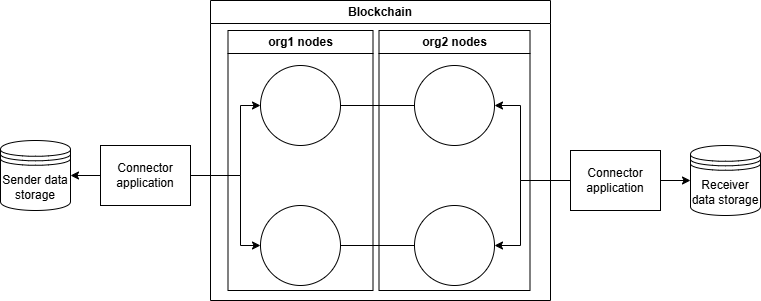
\includegraphics[width=\textwidth]{system_architecture.png}
    \caption{System architecture for two organizations} \label{system_architecture}
\end{figure}

\subsection{SDT process scheme}

The SDT process is presented in Figure \ref{sending_process}.
It represents the following algorithm.

The data transfer process commences with the data sender (Org1) initiating a data transfer request to its connector, which serves as the interface to the blockchain. 
The Org1 connector then persists the data in Org1's storage and gathers associated metadata. 
Subsequently, the Org1 connector queries the blockchain to initiate the execution of the Secure Data Transfer (SDT) smart contract. 
The smart contract validates the provided metadata and records it on the ledger. 
Upon successful metadata validation, the smart contract informs the Org2 connector about the availability of a new message. 
The smart contract also acknowledges the acceptance of the message delivery to Org1.

To retrieve the data, the Org2 connector queries the blockchain nodes and executes the SDT smart contract. 
The smart contract verifies Org2's authorization to access the requested data. 
If authorized, the smart contract requests the data from the Org1 connector. 
Upon receiving the request, the Org1 connector retrieves the data from Org1's storage and transmits it back to the smart contract.

The smart contract then prepares the data for transfer, which may involve encryption and digital signing depending on the specific smart contract implementation. 
The prepared data is subsequently returned to the Org2 connector. The Org2 connector then stores the received data in Org2's storage.

To finalize the process, the Org2 connector notifies the blockchain about the message reception via the smart contract. 
The smart contract updates the message registry, marking the message as delivered. 
The smart contract also notifies the Org1 connector about the successful completion of the message delivery process. 
Finally, the Org1 connector informs the data sender about the completion of the data transfer process.

\begin{figure}
    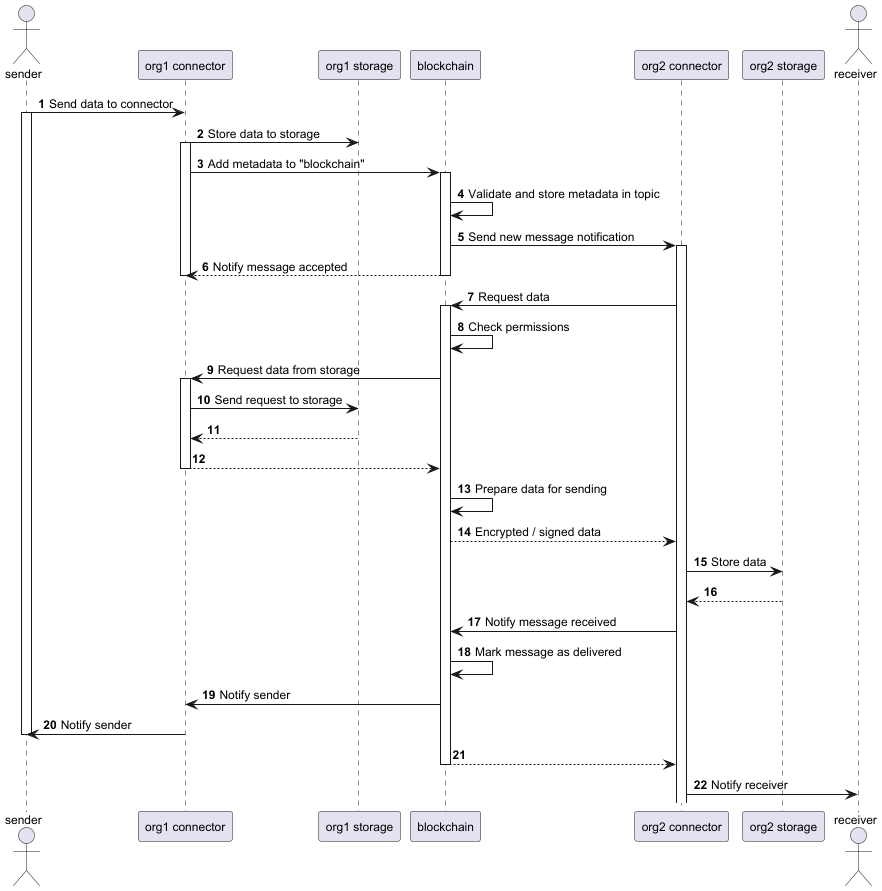
\includegraphics[width=\textwidth]{sending_process.png}
    \caption{SDT process scheme} \label{sending_process}
\end{figure}

Such an algorithm has the following important features:

\begin{enumerate}
    \item Loose coupling between sender and receiver due to blockchain usage as a message broker.
    \item Better fault tolerance compared to regular message brokers.
    \item More convenient message broker-like SDT interface compared to existing blockchain solutions.
    \item Greater SDT process customization capabilities due to smart contract usage.
\end{enumerate}

\section{Implementation details} \label{implementation_details}

\subsection{Blockchain selection}

Blockchain is the core component of the SDT system.
Hence, the particular blockchain implementation has a significant impact on SDT system parameters such as:

\begin{itemize}
    \item Throughput --- the amount of data the system is able to transfer during a fixed time interval.
    \item Fault tolerance --- fault types the system is able to resist and the maximum number of crashed nodes the system is able to handle.
    \item Scalability --- the maximum number of nodes in the system.
\end{itemize}

All parameters presented above depend mainly on the blockchain type and consensus algorithm used.

In the literature reviewed, a notable trend towards private blockchain solutions is observed.
This preference stems from the need for controlled access, enhanced privacy, and potentially higher throughput in many SDT scenarios, particularly in applications like IoT and vehicular networks. 
Several papers mentioned the use of public blockchains, but it was not their primary option. 
Specific examples include:

\begin{itemize}
    \item \cite{Peng2023} proposes a peer-to-peer file storage and sharing system based on a consortium blockchain.
    \item \cite{Jia2023} presents a cross-organizational data sharing framework based on blockchain-probes, implying a permissioned setting.
    \item Several papers addressing IoT applications (e.g., \cite{Ai2022,Gupta2022}) often implicitly or explicitly assume a permissioned blockchain context to address security and scalability constraints.
\end{itemize}

Thus, this paper considers the private blockchain as the best option for SDT system implementation.

In addition to blockchain type selection, it is important to use the correct consensus algorithm.
In order to increase SDT system fault tolerance, this paper proposes PBFT algorithm usage according to the trends observed in the literature.
However, PBFT has known performance limitations.

To start with, PBFT implementations require large volumes of data to be transferred between blockchain nodes in order to achieve consensus.
For example, the BFT-SMaRT algorithm used by Hyperledger Fabric \cite{barger2021byzantine} necessitates the transmission of 80 MB of traffic from each node 
in order to achieve a performance of 2500 transactions per second, which implies the transfer of 720 MB of traffic within a cluster of just 10 nodes during all consensus algorithm stages.

Furthermore, the throughput of such a consensus algorithm depends on the amount of nodes in the system.
According to research \cite{barger2021byzantine}, BFT-SMaRT achieves maximum throughput when the system contains 7 nodes.
Increasing the number of nodes in the system leads to throughput degradation.
The maximum amount of nodes, according to research \cite{Ke2023}, is limited to 100.

For the reasons described above, a pure PBFT blockchain is not suitable for scalable, fault-tolerant systems creation.
Fortunately, this limitation could be solved by using the multi-layered blockchain architecture described in \cite{Bogdanov2024} and \cite{Lin2023} and 
data flow separation into topics and partitions traditional for message brokers like Apache Kafka \cite{apachekafka}.

This paper proposes the usage of the following two-layered blockchain:
\begin{itemize}
    \item The first layer utilizes the PBFT consensus algorithm.
    Due to known algorithm limitations, this layer is to be constructed from many relatively small (up to 7 nodes) clusters.
    This layer represents the concept of a partition --- the smallest system part responsible for message transfer.
    \item The second layer utilizes the RAFT \cite{ongaro2015raft} consensus algorithm.
    This layer is going to be utilized for two main purposes --- system management and asynchronous data replication after PBFT consensus rounds.
    Thus, this layer is analogous to the topic concept of a message broker.
\end{itemize}

Such an architecture allows us to preserve all fault tolerance features provided by the PBFT consensus algorithm while increasing system scalability.
The scaling process of such a system does not require PBFT cluster size growth. 
Instead, a new small PBFT layer 1 cluster is to be created and connected to the existing RAFT layer 2 cluster, which has a relaxed limit on the maximum number of nodes.
\section{Summary} \label{summary}

The paper proposes a novel architecture for secure data transfer (SDT) systems leveraging blockchain technology.
It combines the advantages of two existing paradigms: blockchain as a data access interface and blockchain as a direct data transfer tool.
The architecture features a message broker-like design, overcoming data size limitations of existing blockchain-based SDT solutions.
The proposed system incorporates blockchain, data storages internal to organizations, and connectors that bridge the data storages with blockchain nodes.
The SDT process involves the sender's connector initiating a smart contract on the blockchain, which manages data access, transfer, and confirmation, while the actual data is stored off-chain within the organization's data storage. The paper advocates for a private, two-layered blockchain implementation.
The first layer uses PBFT consensus within smaller clusters for efficient message transfer (partitions), while the second layer employs RAFT consensus for system management and asynchronous data replication (topics).
This layered approach enhances both fault tolerance and scalability.

Further research is going to focus mainly on the following directions:

\begin{enumerate}
    \item Implementation of the proposed system and evaluation of the developed prototype.
    \item Selection of specific consensus algorithm implementations.
    \item Development of a load balancing mechanism for specific partition selection.
\end{enumerate}

\bibliographystyle{splncs04}
\bibliography{references}

\end{document}